\documentclass{report}

\usepackage{graphicx}
\usepackage{amsmath}
\usepackage{amsfonts}
\usepackage{amssymb}
\usepackage[utf8]{inputenc}

\setlength{\textwidth}{18.0cm}
\setlength{\textheight}{23.0cm}
\setlength{\oddsidemargin}{-1.0cm}
\setlength{\evensidemargin}{-1.0cm}
\setlength{\topmargin}{-1.0cm}
\setlength{\parindent}{0pt}

\renewcommand{\baselinestretch}{1.2}
\pagestyle{empty}

\begin{document}

{\it
LULI2000 experiment in Jan 2015 (Al)}

\bigskip

\begin{center}
{\large
\bf
Plasma parameters from FCI2\\[0.2cm]
}
{\it }
\end{center}

\bigskip

{\bf In physical units measured at 2 ns}

\smallskip

$\bullet$ Total magnetic field magnitude : $B_0$ = 60 T \\
$\bullet$ Magnetic ribbon between $L_i$ = 100 $\mu$m \& $L_o$ = 600 $\mu$m. Thickness : $L_t$ = 60 $\mu$m \\
$\bullet$ Electron density $N_0$ = 4 $10^{25}$ m$^{-3}$ (ratio with max density at hot spot = 10) \\
$\bullet$ Total kinetic pressure (mainly from electrons because $Z^{\star}$ = 6) : $P_k$ = 2 10$^{10}$ Pa \\
$\bullet$ Electron temperature (should be the same as ions by collisions) : $T_e$ = 400 eV \\
$\bullet$ Total time of irradiation $T_{\max}$ = 4.0 ns with 0.2 kJ \\
$\bullet$ Proton inertial length : $l_i$ = 36.0 $\mu$m \\
$\bullet$ Proton gyroperiod : $\Omega_i$ = 17.4 ps \\
$\bullet$ Alfvén velocity : $V_0$ = 207 km.s$^{-1}$ \\

\medskip

{\bf In hybrid units (that is at $t$ = 115.0)}

\smallskip

$\bullet$ $T_e$ = 0.9 \ \ --- \ \ $T_i$ = 0.9 \\
$\bullet$ $A$ = 27 \ \ --- \ \ $Z$ = 13 \ \ --- \ \ $Z^{\star}$ = 6 \\
$\bullet$ $L_i$ = 2.8 \ \ --- \ \ $L_o$ = 16.7 \ \ --- \ \ $L_t$ = 1.7 \\
$\bullet$ Asymptotic beta parameter : $\beta_e$ = 1.8 \ \ --- \ \ $\beta_i$ = 0.1 \\
$\bullet$ $\Omega_i$ = 2.1 \ \ --- \ \ $T_{\max}$ = 230.0 \\
$\bullet$ Ion thermal velocity : $v_i$ = 0.18 \ \ --- \ \ ion Larmor radius : $\rho_i$ = 0.37 \\

{\bf Snapshots}

\begin{center}
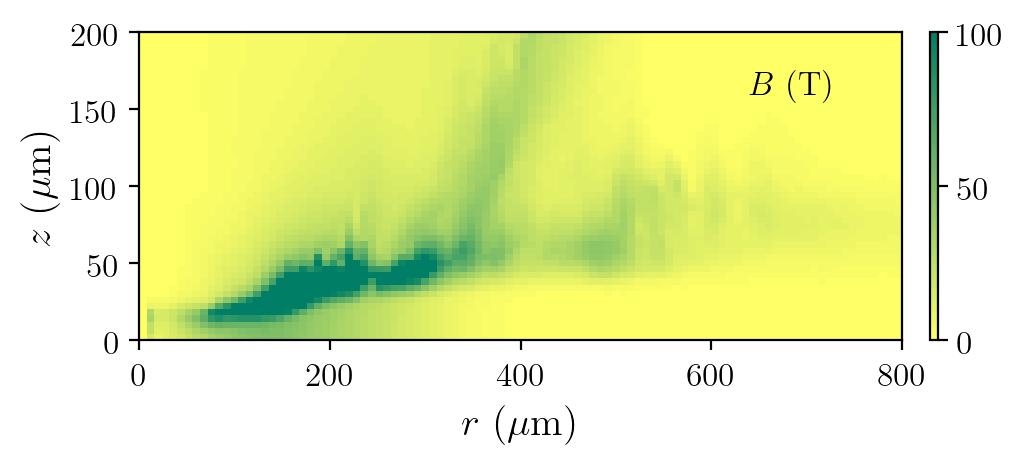
\includegraphics[width=0.8\linewidth]{luli2015_Al-B.png}
\end{center}

\begin{center}
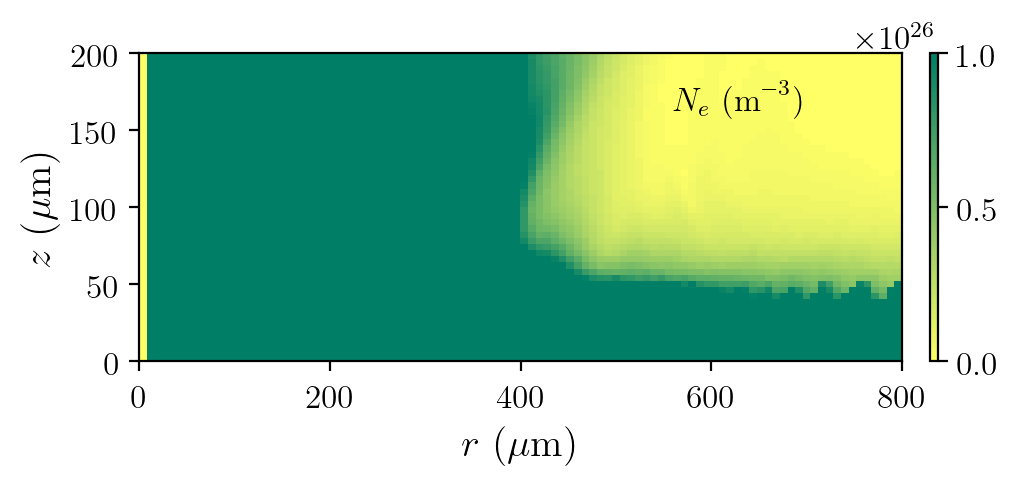
\includegraphics[width=0.8\linewidth]{luli2015_Al-Ne.png}
\end{center}

\begin{center}
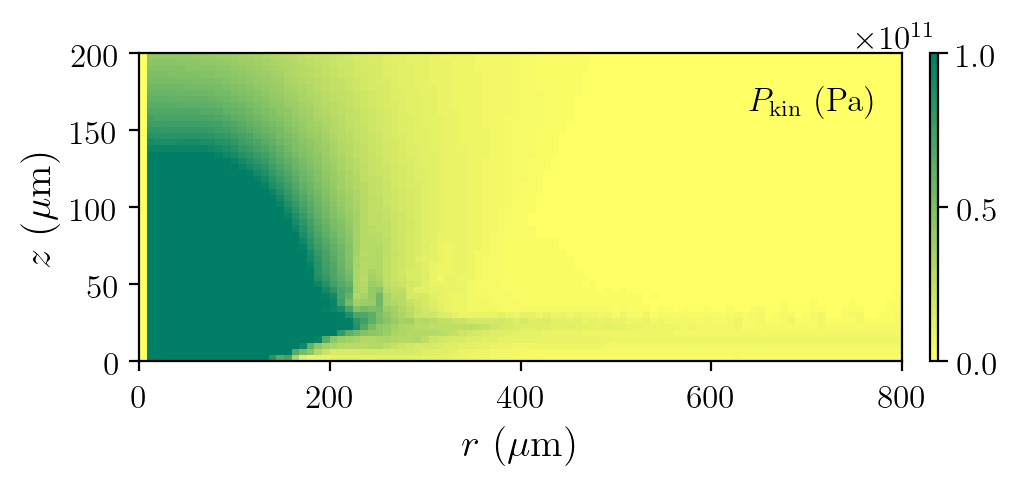
\includegraphics[width=0.8\linewidth]{luli2015_Al-P.png}
\end{center}

\begin{center}
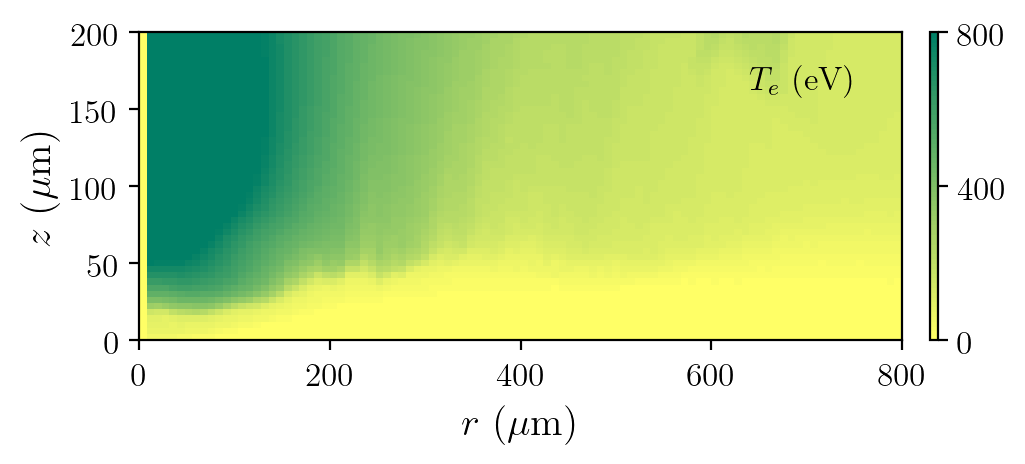
\includegraphics[width=0.8\linewidth]{luli2015_Al-Te.png}
\end{center}


\end{document}
